\section{研究目标与框架基础}
教学回答需要分别核对程序事实和任务完成情况。报对输出不等于解释了学生的误解，合理的讲解也可能给错变式答案。本章研究合成参考能否执行核验并追溯来源、筛选能否减弱表面偏好线索，以及仍有哪些局限。最终交付1000条监督微调（SFT）示范和500对偏好数据，不测量学生学习收益。

\subsection{NaturalThoughts：选择哪些推理示范}
NaturalThoughts包含推理生成与标注、样本选择、监督蒸馏三个环节~\cite{nat}。作者从NaturalReasoning抽取问题，以DeepSeek-R1产生推理轨迹和最终答案；领域、检查与回溯等策略、冗长程度等标注，用于区分多样推理和重复叙述。选择同时考察主题、语义或策略多样性，以及不同推理模型之间的答案分歧等难度代理。分歧不能证明任一答案正确。混合蒸馏为分歧题保留完整推理，其余题可仅保留最终回答，再监督学生模型。

证据具有规模条件：同一Llama-3.1-8B-Instruct在10万条样本下，分歧选择与随机选择的GPQA-Diamond正确率为45.2\%与42.5\%；50万条时则为45.2\%与48.3\%~\cite{nat}（第7页表1）。本项目借鉴分开记录选择属性、另外核验答案的思想，未复现DeepSeek-R1生成、论文标注或大模型蒸馏；结构难度也未按真实学生校准。

\subsection{Matrix：多阶段生产怎样执行}
Matrix将每条输入封装为可序列化的编排对象，保存流程状态、中间历史和路由决策~\cite{matrix}。队列驱动的角色逐步更新并转交对象，完成记录进入持久化输出；模型推理与容器工具由独立服务承担。逐条调度以及数据、任务、角色并行，让样本不必等待整批异质任务结束。系统监测队列、未完成任务和延迟；其至多执行一次语义意味着，角色重启不会自动恢复已出队的执行中样本，必须记录失败并按需离线重跑。

从网页合成推理数据时，文档筛选、题目与参考抽取、独立求解、按需核验是不同步骤。调度机制不决定答案质量，合格标准仍由任务检查给出。论文在相同模型、248张A100、各自并发设置下报告约为Coral的6.8倍吞吐，共识答案正确性指标接近~\cite{matrix}（第9页表1）。本地实现借鉴阶段分离和逐条溯源，没有部署分布式Matrix，也不据此宣称加速。

AIR区分偏好标注、指令选择与回答配对~\cite{air}；fDPO依据当前模型和奖励比较动态过滤~\cite{fdpo}；DEITA结合复杂度、质量和向量多样性~\cite{deita}。这些资料用于解释取舍，未照搬阈值或宣称获得论文中的模型增益。原始机制及结论边界见所引论文。

\begin{figure}[H]\centering
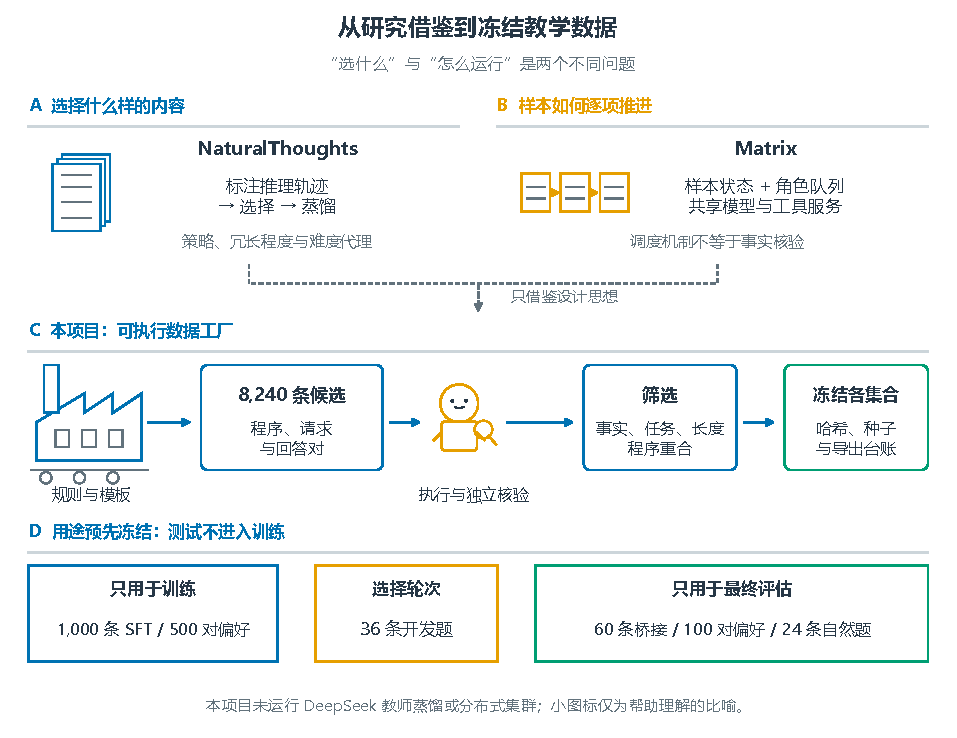
\includegraphics[width=\linewidth]{../../assets/zh/synthesis-atlas.pdf}
\caption{从两套研究框架的启发到可执行数据。框架机制、实际核验和冻结训练／评价导出分别标识。工厂与检验员是解释性比喻，不代表新增智能体或实验对象。}\label{fig:data-pipeline}
\end{figure}\FloatBarrier

\section{可执行数据构建与核验}
SFT记录包含用户与助教消息；偏好记录包含共同请求、首选和次选回答。元数据连接题族、任务、结构难度、种子、候选编号、程序、参考值、筛选去向和导出行号。修订生成器记录8240个候选，训练覆盖24个题族；预测、讲解、诊断、迁移各有250条SFT。500对偏好中，事实错误和指令不符各250对，后者例如遗漏明确要求的解释。这些是按规则构造的对比，并非自然采样的模型错误。冻结文件保持原始中文，没有逐条调用在线教师模型，也没有真实学生观察或教师偏好投票；英文版的例子是译文。

对原程序$P$及变式$P'$，独立计算的参考$y,y'$须满足
\begin{equation}
V(P,P')=\mathbf1\{\operatorname{stdout}(P)=y\}\mathbf1\{\operatorname{stdout}(P')=y'\}.
\label{eq:data-exec}
\end{equation}
独立核验脚本仅用标准库，不导入生成器或渲染器；检查明确标记的参考及负例类型，要求应改变答案的变式确实改变。跨集合核对规范化程序和请求，包括原题／变式的所有组合。另一粗粒度AST指标去除变量名与常量，用于暴露模板重复，与精确去重的目的不同；共同项目作者身份仍限制了独立性。

导出包括1000条SFT、500对训练偏好、三个留出题族的36条开发示范、逐字节保留的60条旧版桥接参考、100对偏好测试和24道另行编写的自然题。开发集选检查点，测试不参与。自然题由项目内Codex编写，部分主题与训练重合，检验新实例和问法，不代表全新知识。修订核验通过11234项异质检查，10个主要文件可逐字节再生；它支持可执行一致与溯源，不能解释为11234次教学评分通过。

\section{筛选对照与剩余捷径}
原版在同一1931对合格偏好候选上进行受控选择。50个共同排列比较随机选择A、任务／背景／缺陷均衡B、再加入长度优先C，各题族配额固定，每次均取500对；未打乱的C复现正式编号。50次只是同一候选池的顺序置换，并非独立采集。定义“总选长回答”的命中率
\begin{equation}
H=(n_{\mathrm{preferred\ longer}}+0.5n_{\mathrm{equal}})/N.
\label{eq:data-heuristic}
\end{equation}
标签偏差$D$为任务、背景、缺陷三轴上，族内频率与均匀分布总变差距离$\frac12\sum_k|p_k-1/K|$的配额加权均值。

\begin{table}[H]\centering\small
\caption{固定候选池的筛选：均值（50次置换样本标准差），$D$仅列均值。}\label{tab:data-ablation}
\begin{tabularx}{\linewidth}{@{}Yrrr@{}}\toprule
策略 & 首选较短（\%） & 选长命中$H$（\%） & $D$\\\midrule
A：随机 & 19.08（1.43） & 80.63（1.44） & 0.1112\\
B：标签均衡 & 19.39（1.03） & 80.31（1.02） & 0.0189\\
C：长度与标签 & 43.89（0.12） & 55.97（0.15） & 0.0278\\\bottomrule
\end{tabularx}
\end{table}\FloatBarrier

\begin{figure}[H]\centering
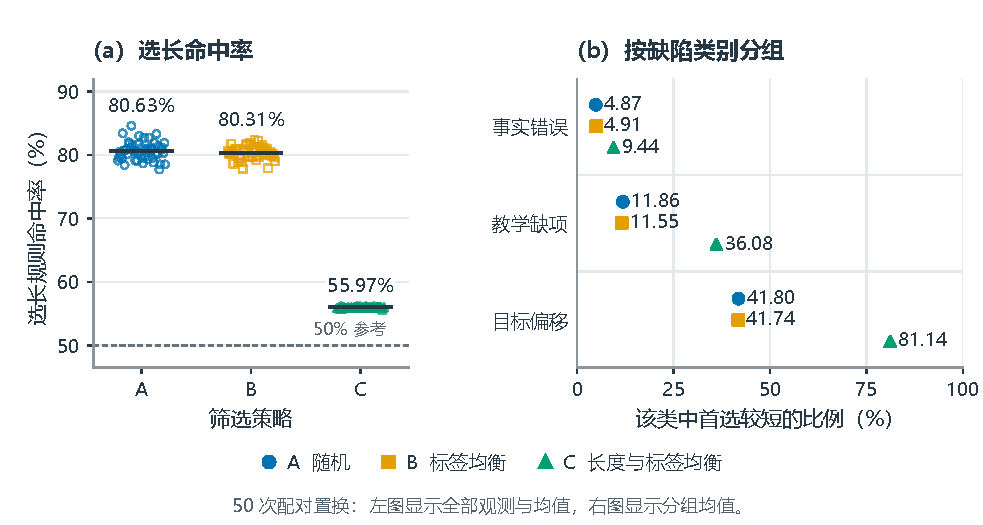
\includegraphics[width=\linewidth]{../../assets/zh/selection-ablation.pdf}
\caption{三种策略下实际可测的长度线索。散点保留50次配对置换，分类均值揭示总体均衡掩盖的差异。此对照没有训练模型。}\label{fig:data-ablation}
\end{figure}\FloatBarrier

C相对B在每次置换中均降低$H$：平均减少24.34个百分点，标准差1.02，范围为减少21.7至26.3个百分点；但$D$由0.0189升到0.0278，存在取舍。C的分类首选较短比例仍为事实错误9.44\%、教学缺项36.08\%、目标偏移81.14\%。

题族供给解释了为何不能按族各半得到250对较短首选：向下取整目标总计245，列表别名、循环控制、递归分别缺14、7、5对；七个奇数配额题族可各多取一对。因此各族尽量近半的总数范围是219--226，正式集220对，置换219--221对。整体取250对仅能通过部分题族补偿其他题族、偏离族内各半实现。

\begin{figure}[H]\centering
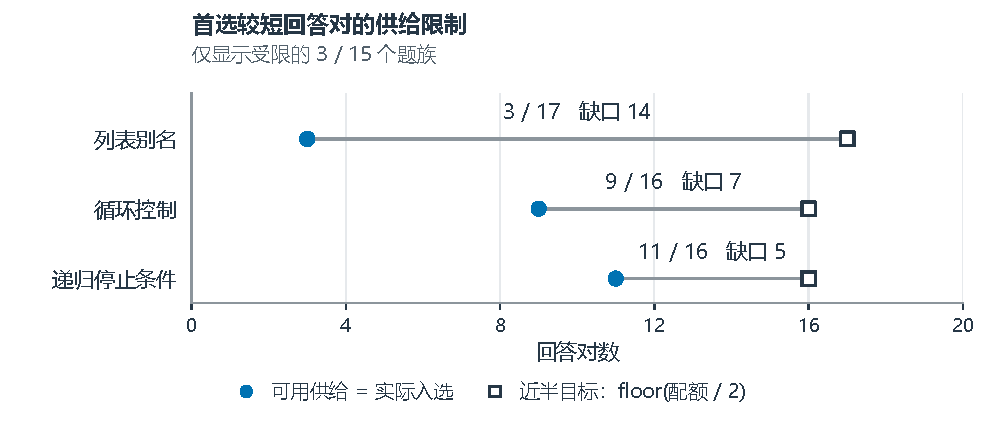
\includegraphics[width=\linewidth]{../../assets/zh/family-supply.pdf}
\caption{原15个训练题族中，三个题族的较短首选供给不足以达到配额一半的向下取整值；它们的全部可用较短首选均已入选，标注缺口给出约束来源。}\label{fig:data-family-supply}
\end{figure}\FloatBarrier

原版179条偏题次选还含互斥固定片段：58条有\verb|sep='-'|，62条有\verb|end=''|，59条有\verb|print('A#B')|；其余321条次选和500条首选均不匹配。修订删除这些已知线索并缩短回答，不能据此证明全部捷径消失。

\begin{table}[H]\centering\small
\caption{同口径正式发布集诊断。55.9\%是正式集结果，区别于55.97\%的置换均值。}\label{tab:data-revision}
\begin{tabularx}{\linewidth}{@{}Yrr@{}}\toprule
指标 & 原版 & 修订版\\\midrule
SFT／偏好AST结构数 & 105／98 & 145／121\\
SFT／首选字符中位数 & 306／296 & 65／64\\
选长回答命中率 & 55.9\% & 50.0\%\\
匹配已检固定片段的次选 & 179 & 0\\\bottomrule
\end{tabularx}
\end{table}\FloatBarrier

剩余耦合仍强：250条事实错误负例中，迁移122、诊断121、预测6、解释1；250条指令不符则全部来自预测／解释，偏好测试也有类似关联。1000条SFT均恰含一次固定输出标签，只对应145种结构和890种完整回答；36条开发示范仅四种结构。可执行并不等于教学与协议覆盖充分。

\section{结论与补充证据}
数据研究完成生成与筛选交付，并测量了特定表面线索的变化，没有证实推理改善、教师认可或学习收益。历史12例抽查属于非盲Codex检查，不能估计全库教学成功率。候选流量、不同指纹口径、逐条审阅及完整C00670偏好样本保留在数据与对照记录中。第二章实际检验更强的模型可靠性命题。

\begin{quote}\small\textbf{阅读注释。} 可以把SFT看作示范教材，把偏好对看作同题两种回答的比较。“首选”既可能因为算对，也可能因为更符合请求；不是越长越好。程序核验像检查答案的尺子，不能代替教师判断讲解是否有效。
\end{quote}
